\chapter{Example}
\label{ch:example}

!!! Please delete this chapter after finishing your work !!!

\section{Settings}

To add your name and the title of your work, please use the ``Settings.tex'' file!
Additionally, switch there between German and English version.

\section{How to Make Sections and Subsections}

Use section and subsection commands to organize your document. \LaTeX{} handles all the formatting and numbering automatically. Use ref and label commands for cross-references.

\subsection{How to Make Lists}

You can make lists with automatic numbering \dots

\begin{enumerate}
\item Like this,
\item and like this.
\end{enumerate}
\dots or bullet points \dots
\begin{itemize}
\item Like this,
\item and like this.
\end{itemize}
\dots or with words and descriptions \dots
\begin{description}
\item[Word] Definition
\item[Concept] Explanation
\item[Idea] Text
\end{description}

\section{Section}

You have to write text between each headline.

\section{Citation}

This part describes the three types of citations which are possible:

\section{Direct Citation}

The maximum for a direct citation is a ${1/2}$ page.

\begin{quotation}
	Overview first, zoom and filter, then details-on-demand
	\autocite{shneiderman_eyes_1996}
\end{quotation}

\section{Floating Text Citation}

\textcite{shneiderman_eyes_1996} defined the Visual Information Seeking Mantra as ``Overview first, zoom and filter, then details-on-demand''.

\section{Indirect Citation}

Some text which summarizes a paper or a book chapter. This could take several lines.
Find attached a citation of a website~\autocite{kaley_match_2018}.

\newpage
\section{Figures}

To place a figure use the following code example

\begin{figure}[ht!]
  \centering
  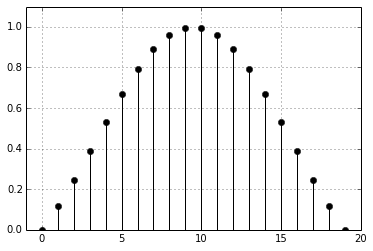
\includegraphics[width=1\columnwidth]{Figures/Example}
  \caption{Interactive data exploration with multiple devices.}
  \label{fig:example}
\end{figure}




\begin{figure}[h]
    \centering
    \subfigure[Figure A]{
    	\label{fig:a}
        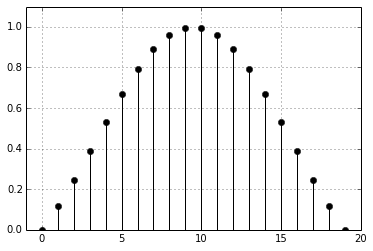
\includegraphics[width=60mm]{Figures/Example}
     }
	\subfigure[Figure B]{
    	\label{fig:b}
        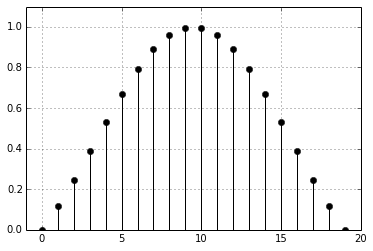
\includegraphics[width=60mm]{Figures/Example}
     }
    \caption{Wearables worn for experiments 1, 2, and 3.}\label{fig:figure2}
\end{figure}

Refer to a figure in the following forms:\\
If you take a look at Figure~\ref{fig:example} ...\\
... text text (see Figure~\ref{fig:example}) ...

\section{Listings}
\begin{lstlisting}[caption=A bit of source code., label=lst:test]
if( true == questions )
{
    std::cout << "Let me google it for you";
}
else
{
    std::cout << "Great";
}
\end{lstlisting}

Now lets take a look at Listing~\ref{lst:test}.


\section{Table}

\begin{table}[ht!]
  \caption{My caption with a very useful description. die kann auch etwas länger sein und über mehrere Zeilen gehen und so weiter.}
  \label{my-label}
  \begin{tabular}{llr}
    \hline
    \multicolumn{2}{c}{Item} &            \\ \cline{1-2}
    Animal     & Description & Price (\$) \\ \hline
    Gnat       & per gram    & 13.65      \\
               & each        & 0.01       \\
    Gnu        & stuffed     & 92.50      \\
    Emu        & stuffed     & 33.33      \\
    Armadillo  & frozen      & 8.99       \\ \hline
  \end{tabular}
\end{table}

For the fast generation of tables from Excel use \url{http://www.heise.de/download/excel2latex.html}

\section{Equations}

\LaTeX{} is great at typesetting equations. Let $X_1, X_2, \ldots, X_n$ be a sequence of independent and identically distributed random variables with $\text{E}[X_i] = \mu$ and $\text{Var}[X_i] = \sigma^2 < \infty$, and let

$$S_n = \frac{X_1 + X_2 + \cdots + X_n}{n}$$

This was a equation without a label.
      
\begin{equation}
S_n = \frac{1}{n}\sum_{i}^{n} X_i
\label{eq:test}
\end{equation}

This is the reference to equation~\ref{eq:test}.      

denote their mean. Then as $n$ approaches infinity, the random variables $\sqrt{n}(S_n - \mu)$ converge in distribution to a normal $\mathcal{N}(0, \sigma^2)$.


